\section{Cancer}
\label{intro-sec:cancer}

While cancer is a massively heterogenous disease, as it can arise through a multitude of ways in almost any tissue, there are a some fundamental defining features, which most, if not all malignancies acquire, before they are truly cancers . The original characteristics comprise 
\begin{enumerate*}
	\item Sustaining proliferative signaling
	\item Evading growth suppressors
	\item Activating invastion and metastasis
	\item Enabling replicative immortality
	\item Inducing angiogenesis
	\item Resisting cell death
\end{enumerate*} (\autoref{fig:oldhallmarks}). 
These hallmarks were long considered the core of tumour development and the authors themselves hypothesised, that these core mechanics allow us to condense the complexity that cancer displays, both in the clinic as well as in labs, with a small set of rules, which all cancers have to obey \cite{Hanahan2000}. In their exact words: ``We foresee cancer research developing into a logical science, where the complexities of the disease, described in the laboratory and clinic, will become understandable in terms of a small number of underlying principles``

\begin{figure}[!ht]
\centering
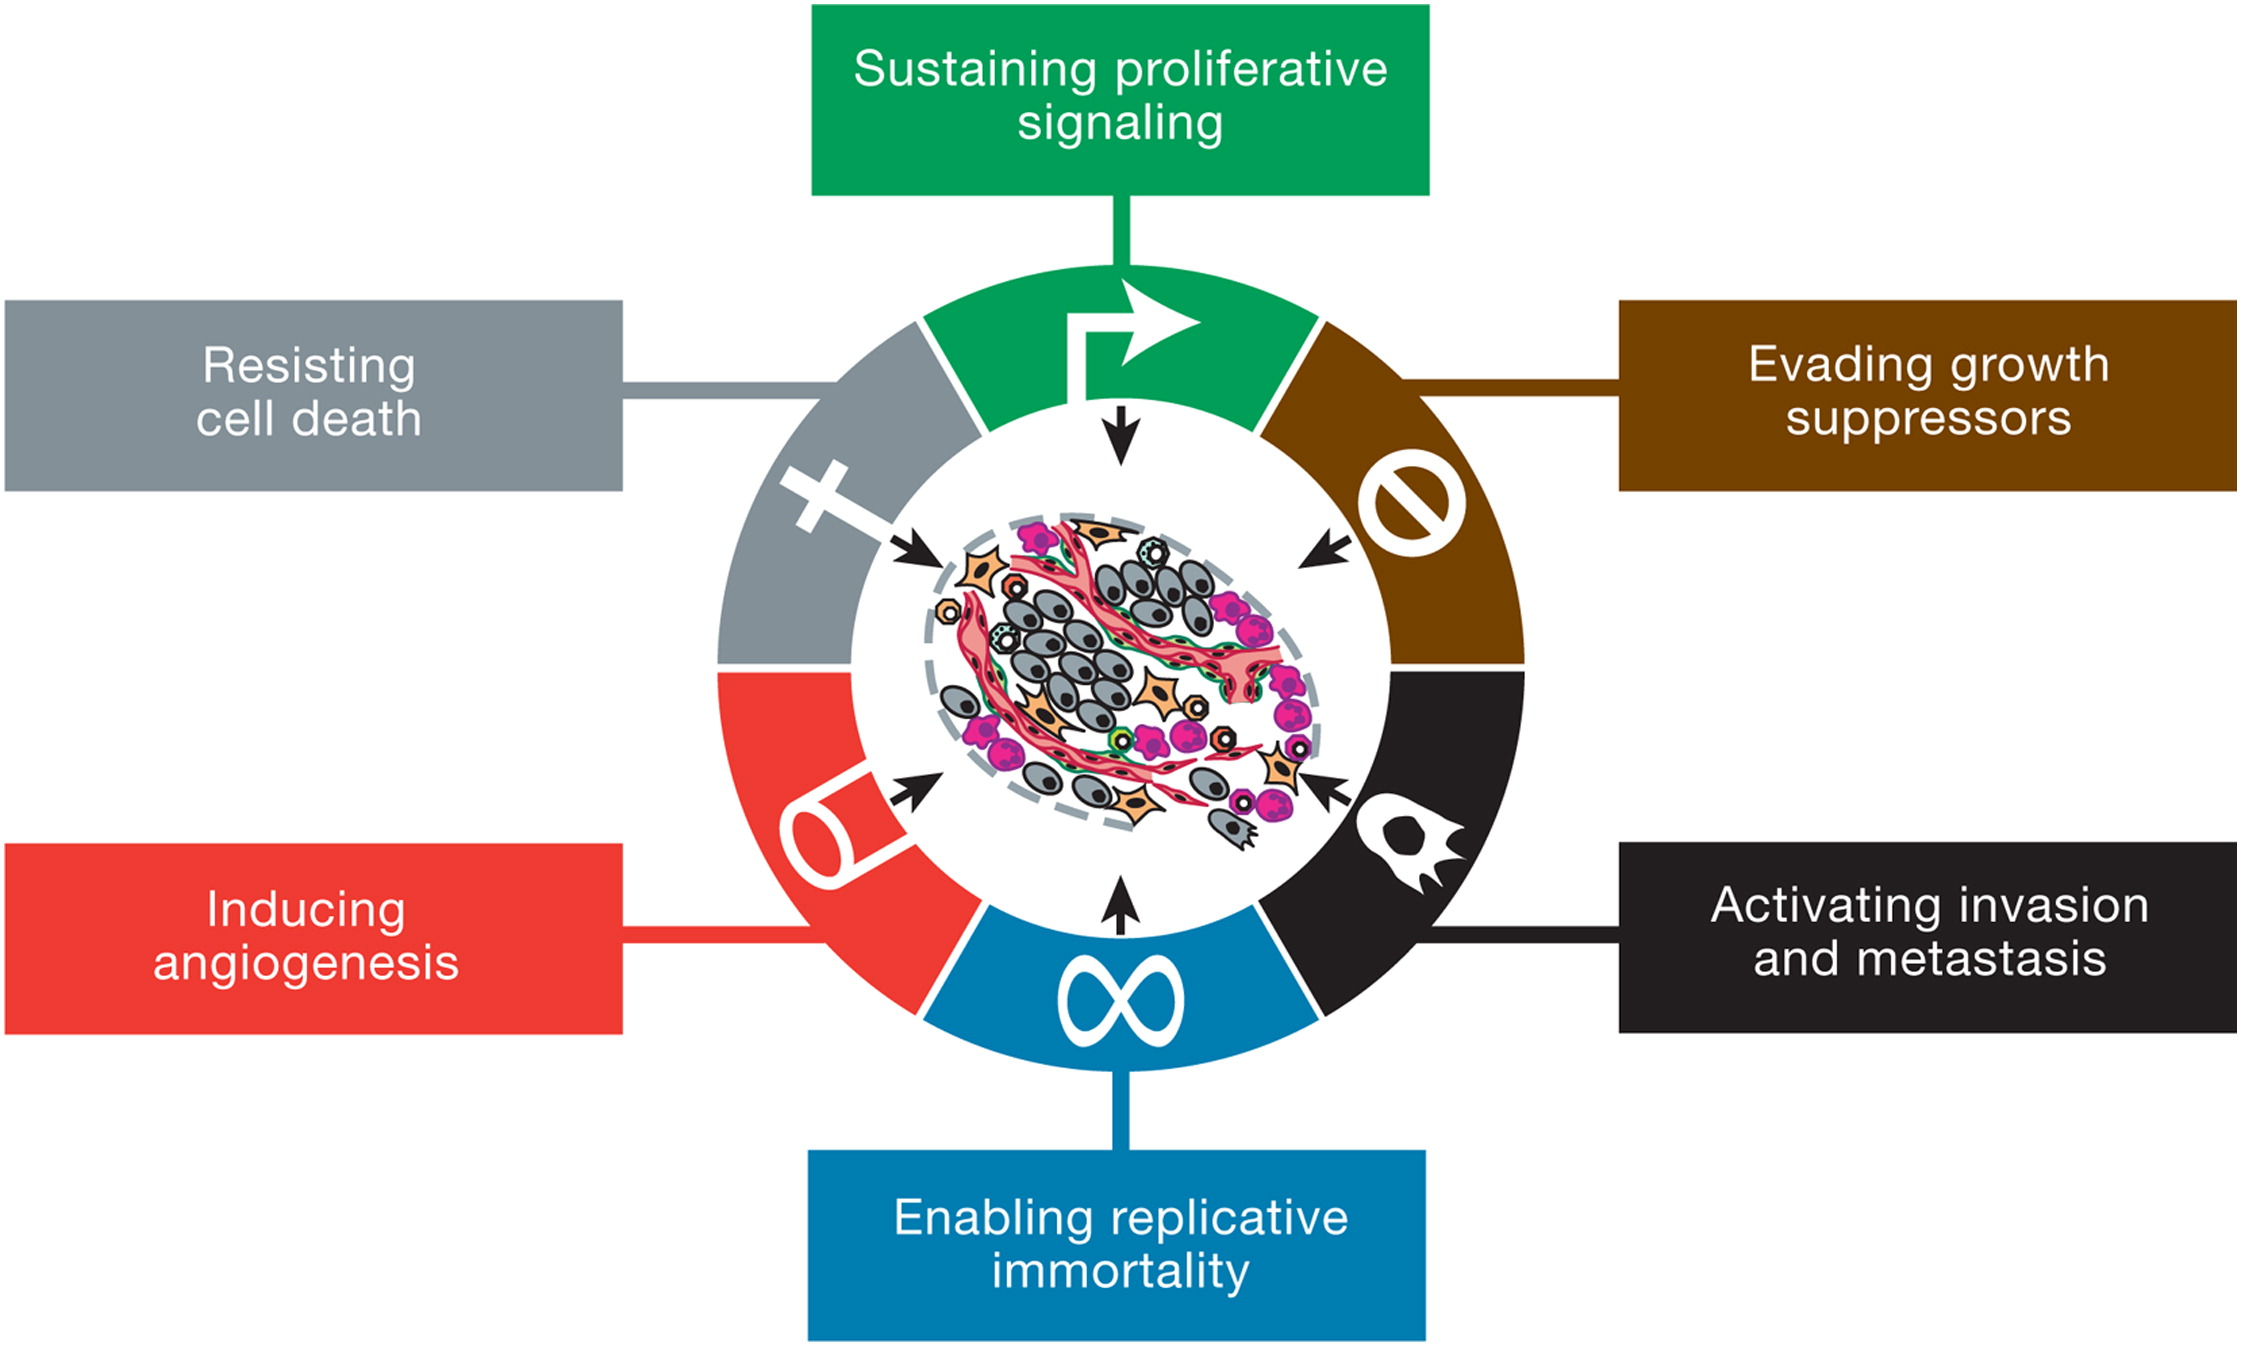
\includegraphics[width=.95\linewidth]{Figures/oldHallmarksCancer.jpg}
\caption[Original hallmarks of cancer]{Acquired capabilities of cancer; Functional capabilities acquired by most cancers during their development; Figure adapted from \protect\citeauthor*{Hanahan2000}\protect\cite{Hanahan2000}}\label{fig:oldhallmarks}
\end{figure}

However, with 11 years of additional research into the topic, more hallmarks have been found and the original list was revised by the authors to contain additional characteristics, namely 
\begin{enumerate*}
\item Avoiding immune destruction
\item Tumour-promoting inflamation
\item Genome instability and mutation
\item Deregulating cellular energetics
\end{enumerate*}
(\autoref{fig:newhallmarks}) \cite{Hanahan2011}. And even then a few years later, even more hallmarks e.g. metabolic rewiring are now considered a part of the characteristics of cancer \cite{Fouad2017}.

\begin{figure}[!ht]
\centering
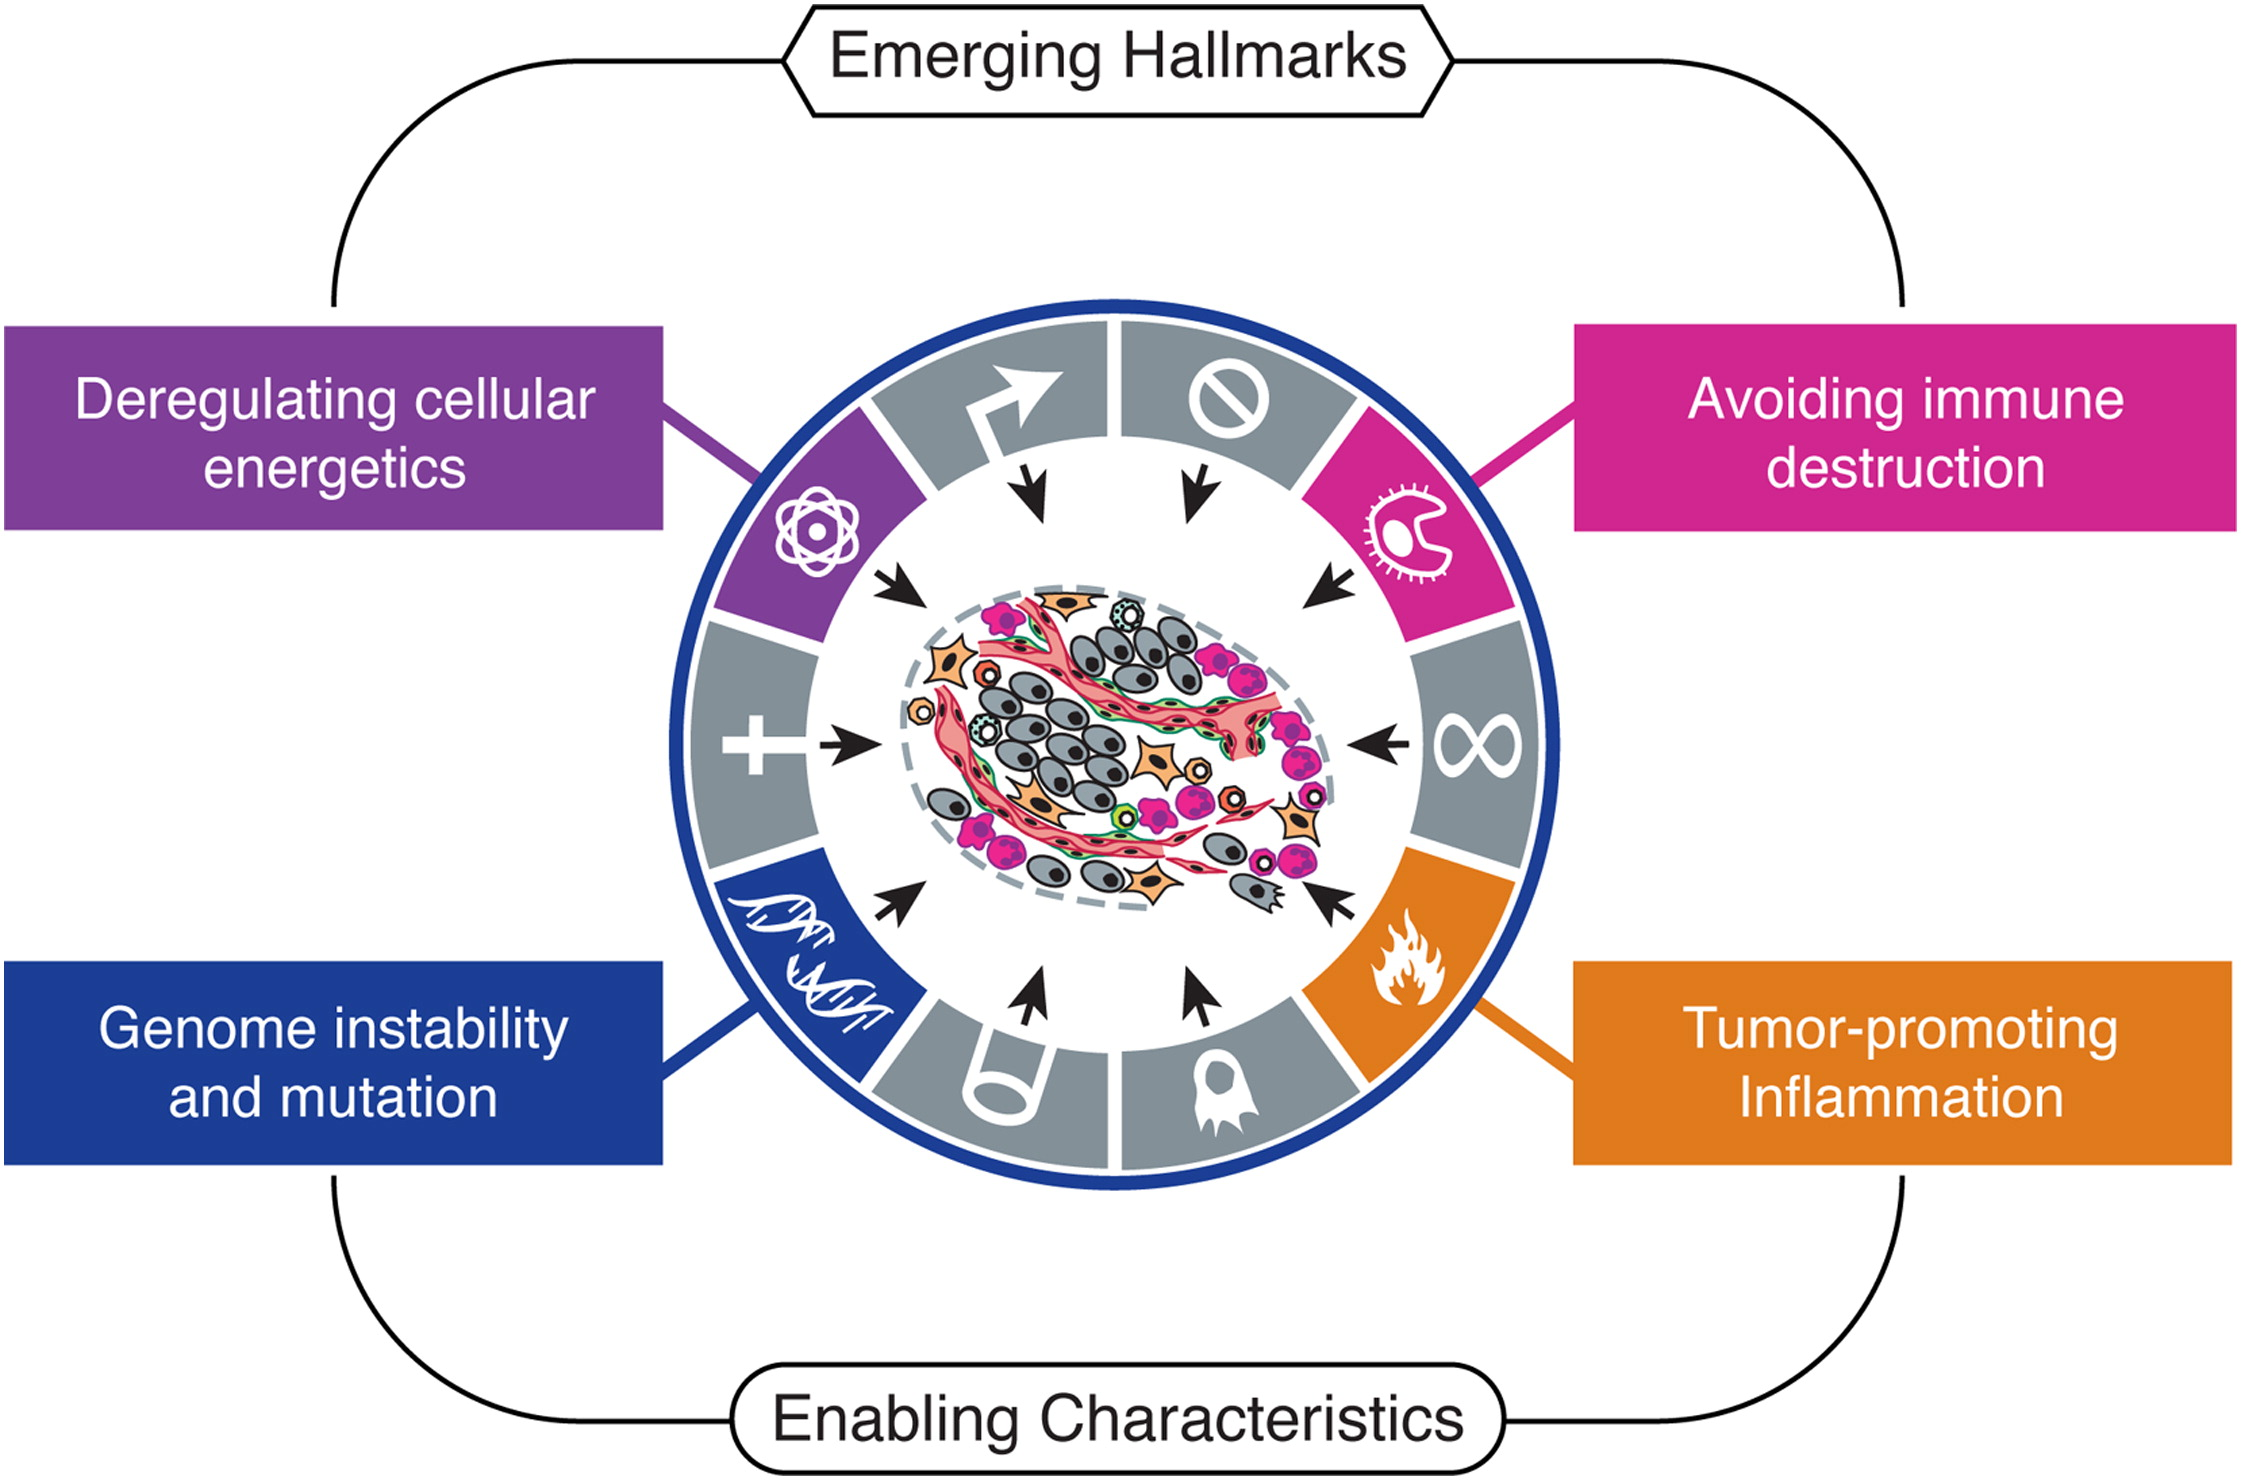
\includegraphics[width=.95\linewidth]{Figures/newHallmarksCancer.jpg}
\caption[New hallmarks of cancer]{Emerging hallmarks and enabling characteristics of cancer; updated version of the hallmarks figure (\autoref{fig:oldhallmarks}) with ; Figure adapted from \protect\citeauthor*{Hanahan2011}\protect\cite{Hanahan2011}}\label{fig:newhallmarks}
\end{figure}

So while the original set of the hallmarks was not sufficient or complete, it offered a good attempt at abstraction of biological concepts to describe cancers. In the following pages, I will outline each of those hallmarks and how it influences my research.

\todo[inline, color=red]{describe the hallmarks}

\subsubsection{Sustaining proliferative signaling - there are no breaks on the train}

\subsubsection{Evading growth suppressors}

\subsubsection{Activating invasion and metastasis - look at me... I am the organism now}

\subsubsection{Enabling replicative immortality}

\subsubsection{Inducing angiogenesis}

\subsubsection{Resisting cell death}

\subsection{Lungcancer}
\label{intro-sec:lungcancer}

With around 1.6 million deaths world-wide each year, lung cancer is the number one cause of cancer death \cite{Siegel2018}. Every year about twelve thousand Australians get diagnosed with lung cancer. These cases can be generally split into two groups: small cell lung cancers (SCLC) and non-small cell lung cancers (NSCLC), which account for around 15\% and 85\% of cases, respectively. The majority of NSCLC are either lung adenocarcinoma or lung squamous cell carcinoma \cite{Molina2008}. Even though smoking is highly associated with lung cancers, there is a big group of never smokers, with a high risk of lung cancers in East Asia, especially women, which is correlated with outside influences like pollution and occupational carcinogens and paired with genetic susceptibility \cite{Sun2007}.
This group usually shows \textit{EGFR} (epidermal growth factor receptor) driven tumours. EGFR is a transmembrane receptor tyrosine kinase, which is usually only expressed in epithelial, mesenchymal, and neurogenic tissue, but its overexpression in other tissues is a hallmark of many human malignancies, not just NSCLC.

\todo[inline]{Possibly change this to cancer in general}

%% original abstract
%Approximately 50% of patients with non-small cell lung cancer (NSCLC) develop acquired resistance to EGFR tyrosine kinase inhibitors (TKIs) through mutations in EGFR T790M. Maintaining a dynamic balance between T790M positive and negative clones offers an opportunity to delay the emergence of resistance and improve disease outcomes. It is now possible to quantify EGFR mutations using circulating tumour DNA (ctDNA) which can provide a surrogate measure of clonal populations within tumours. This project will utilise next generation sequencing (NGS) of tumour tissue and ctDNA in patients treated with EGFR TKIs to study clonal evolution patterns and predict optimal treatment approaches to delay therapeutic resistance.